\documentclass[12pt]{article}
\usepackage{amssymb,amsmath,graphicx,mathtools}
\usepackage{listings}
\usepackage[margin=0.75in]{geometry}
\parindent 16 pt
\usepackage{fancyhdr}
\usepackage[hidelinks]{hyperref}
\usepackage{url}
\usepackage[usenames,dvipsnames]{xcolor} % Required for custom colors
\usepackage{listings}
\usepackage{float}
\usepackage{sectsty}
\usepackage[bottom]{footmisc}
%\pagestyle{fancy}
%\fancyhead[R]{Imad Ali}
%\fancyhead[L]{Bayesian Win Probability in Basketball}
\DeclarePairedDelimiter\ceil{\lceil}{\rceil}
\DeclarePairedDelimiter\floor{\lfloor}{\rfloor}

\sectionfont{\sffamily\bfseries\upshape\large}
\subsectionfont{\sffamily\bfseries\upshape\normalsize}
\subsubsectionfont{\sffamily\mdseries\upshape\normalsize}

\definecolor{links}{HTML}{FF6688}

\lstset{
    language=R,
    basicstyle=\scriptsize\ttfamily,
    stepnumber=1,
    numbersep=5pt,
    showspaces=false,
    showstringspaces=false,
    showtabs=false,
    frame=single,
    tabsize=2,
    captionpos=b,
    breaklines=true,
    breakatwhitespace=false,
    escapeinside={},
    keywordstyle={},
    morekeywords={}
    }

\title{Bayesian Alternatives to Statistical Significance}
\author{Imad Ali\thanks{National Basketball Association} \and Jonah Gabry\thanks{Columbia University}}

\begin{document}
\maketitle
\abstract{\noindent This paper outlines common misconceptions of Frequentist ``statistical significance'' and proposes a more intuitive Bayesian alternative. At a high level, Frequentist methods focus on the distribution of the test statsitic (which is computed from the parameter of interest), whereas the Bayesian methods proposed here allow the researcher to perform inference directly on the parameter of interest.}
\tableofcontents
\newpage
% CaUSTOM SHORTCUTS

\def\ci{\perp\!\!\!\perp}
\def\ex{\mathbb{E}}
\def\prob{\mathbb{P}}
\def\ind{\mathbb{I}}
\def\grad{\triangledown}
\def\bigo{\mathcal{O}}

\section{Introduction}

As applied researchers, we are sometimes interested in determining whether an estimate computed from a sample of data (e.g. the mean) is different from some hypothesized value. In Frequentist methodology, the appropriate way to test for a statistically significant difference between the mean of the data and some hypothesized value is to implement a t-test. There is plenty of literature that discusses hypothesis testing and delves into the derivation and math behind the t-test and the associated p-value. Kruschke (2015) provides an overview of hypothesis testing along with a Bayesian approach, which involves computing the highest density interval. This interval is simply the application of quantiles to the posterior distribution (where the probability values are defined at the researchers discretion). \\

\noindent In this paper we seek to build a better understanding about what the t-test is doing by taking a more empirical approach to constructing the test under the Frequentist framework. Through the application of quantiles we also show how to perform a more intuitive Bayesian test that can be applied to both the parameters and the posterior predictions. \\

\noindent In the remainder of this section we discuss common misconceptions surrounding test statistics, p-values, and generally speaking the misuse of the term statistical significance. The following section discusses what statistical significance and p-values mean using the one sample t-test as an example. We then show an alternative approach to both the one sample and two sample t-test using the Bayesian framework to evaluate a meaningful difference in parameters.\footnote{We use the term \emph{meaningful} instead of \emph{significant} to avoid confusion since the latter term as been adopted by Frequentists to imply a meaningful difference in parameters.} We extend this further to show how inference on posterior predictions can be more important than inference on the parameter estimates. The appendix outlines how the Bayesian approach to the one sample t-test can be extended to two samples as well as the Binomial test. \\

\subsection{Misinterpreting statistical significance}

\noindent A quantity is defined to be statistically significant if the test statistic computed with this quantity is unlikely to occur under the null hypothesis, where the null hypothesis assumes that there is no difference between the quantity and its hypothesized value (this is known as a two-tailed test).\footnote{In some situations the researcher might be interested in whether the quantity is greater/less than some hypothesized value, in which case a one-tailed test is more appropriate.} What this means is that if we repeatedly draw samples from the population under the null hypothesis, compute the same statistic, and plot the empirical distribution of the statistic; then the statistic we computed from our original data would fall somewhere in the tails of this distribution (i.e. a low probability region). A common approach to quantify this is to compute the proportion of the distribution that is in the tails from the computed test statistic. This quantity is known as a p-value and tells you the probability of computing a statistic under the null hypothesis that is as extreme as the one at hand. Lower p-values indicate that the computed test statistic is way out in the tail(s) of the distribution, and thus is unlikely to occur under the null hypothesis. \\

\noindent In this discussion of statistical significance we have been talking about quantities that we, as applied researchers, are not really interested in; test statistics and p-values. We are more interested in the underlying quantities used to compute these statistics (in the case of a one sample t-test this is the mean of the data). \\

\section{Inference on Sample Parameters}

\noindent It is easier to talk about the process of inference in context so we will use the one sample t-test is used as an example. First we will show how statistical significance is determined using the t-test and then we will outline a Bayesian alternative by modeling the data using \textbf{rstanarm}, a high level R interface for regression modeling with Stan (a probabilistic programming language). \\

\noindent Below we have a sample of ten observations $x$ generated from $\mathcal{N}(\mu = 4.5, \sigma = 2)$. The parameter $\mu$ is the population mean and the parameter $\sigma$ is the population standard deviation.

\begin{verbatim}
            x <- c(5.820883, 2.667825, 3.332511, 3.388233, 7.976444,
                   5.925112, 6.465919, 7.064625, 3.012066, 2.771472)
\end{verbatim}

\noindent Recall that population parameters are typically unknown. What is known is the sample mean $\mu_s$ (which is the mean of $x$) and the sample standard deviation $\sigma_s$ (which is the standard deviation of $x$).

\subsection{One Sample t-test}

The \emph{one sample t-test} is used to test the whether the mean of a sample of data $\mu_s$ is significantly different from some hypothesized value $\mu_0$. Note that $\mu_0$ is some hypothesized value chosen by the researcher whereas $\mu$ is (typically) unknown. The test statistic associated with this test assumes that data $x$ is generated from the normal distribution and is calculated as,

$$
\mbox{t-statistic} = \frac{\mu_s-\mu_0}{\sigma_s/\sqrt{n}}
$$

\noindent where $\sigma_s$ is the standard deviation of the data $x$ and $n$ is the sample size of the data. This statistic follows the t-distribution with $n-1$ degrees of freedom. \\

\noindent Suppose we want to test whether the mean of the data is statistically different from a hypothesized value $\mu_0 = 4.5$. This is a two-tailed test since we are interested in determining whether the mean is significantly greater than 4.5 or significantly less than 4.5. Applying the t-statistic formula to the data yields the following value,

$$
\frac{4.84-4.5}{2.01/\sqrt{10}} \approx 0.5394
$$

\noindent Since we are dealing with a two-tailed test our test statistics of interest are $\mid 0.5394 \mid$ and $-\mid 0.5394 \mid$. As mentioned in the introduction, we want to determine how unlikely it is to compute test statistics more extereme than the one we have computed. This is done by using the cumulative distribution function for the t-distribution $F(q, \nu)$ parameterized by quantity $q$ and degrees of freedom $\nu$. Since the t-distribution is symmetric we can compute the probability of calculating a statistic less than or equal to -0.5394 under the null hypotheis and multiply this value by 2 (to account for the fact that we are performing at two-tailed test). Performing this computation yields,

$$
2 \cdot F(0.5394, 10-1) \approx 0.6027
$$

\noindent So there is about a 0.6 probability that a test statistic could occur that is more extereme than the one we computed. In other words, if we repeatedly randomly sample 10 observations under the null hypotheis $x \sim \mathcal{N}(4.5, 2)$ and compute the t-statistic with this data, then 60\% of the time we will observe t-statistic values more extreme than what we calculated with the orginal data sample. That is a high probability and suggests that there may be no difference between the test statistic computed from the data sample and the test statistics computed under the null hypothesis. Under the Frequentist interpretation, this implies that the mean of our sample is not statistically different from the hypothesized value, 4.5. \\

\noindent The distribution of t-statistics under the null hypothesis can be illustrated by sampling 10 observations from $\mathcal{N}(4.5,2)$ $B$ times, and plotting a histogram of these $B$ t-statistics. The figure below illustrates such a histogram where $B = 10,000$.

\begin{figure}[H]\caption[]{Empirical Distribution of t-Statistic}
\centering
\begin{minipage}{0.6\linewidth}
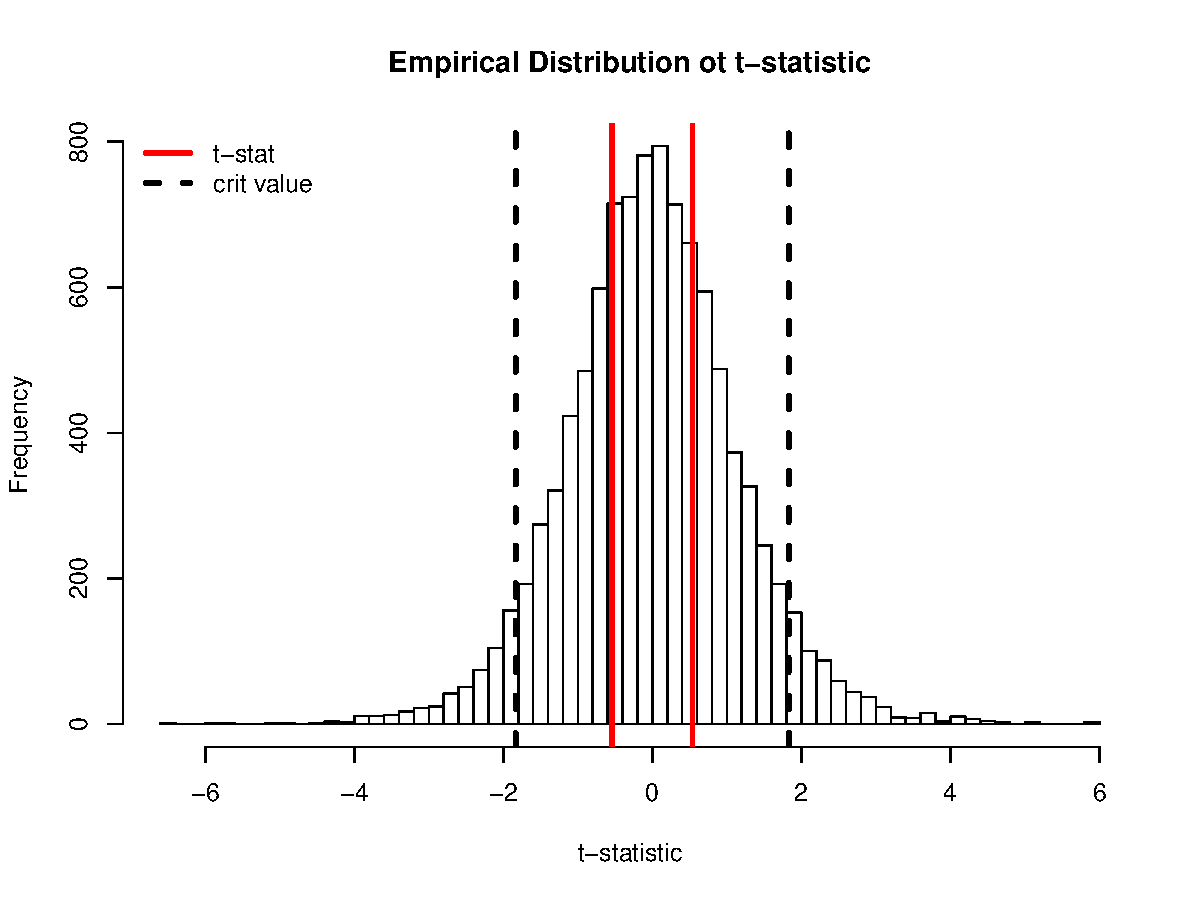
\includegraphics[trim={0cm 0cm 0cm 1.5cm}, clip, scale=0.6]{../figs/ttest_dist.pdf}
\end{minipage}
\end{figure}

\noindent The red lines indicate the t-statistic computed with the data sample provided above. The dashed black lines indicate the critical values where the proportion of the distribution in the tails from those dashed lines is cumulatively 0.1.\footnote{The choice of 0.1 is arbitrary (0.05 is often used in Frequentist literature). The researcher should choose the threshold that is appropriate given the context of the problem.} If our computed t-statistic is outside the critical values then we could say that there is less than 0.1 probability that we would calculate a statistic as extreme as the one we have calculated, suggesting that the statistic is somewhat unique. This would tangentially indicate that there is a significant difference between the mean of our data $\mu_s$ and the null hypothesis $\mu_0$. However the statistic falls inside the critical value interval, which leads to the conclusion that $\mu_s$ is not statistically different from 4.5. \\

\subsection{Bayesian alternative to the one sample t-test}

The approach above focused on the test statistic which is derived from the parameter of interest $\mu_s$. The Bayesian alternative to this test involves modeling the data with prior information, and performing inference directly on the parameter estimate $\mu_s$. \\

\noindent In the context of the t-test assumptions the data is modeled using the normal distribution. The prior distributions on the location and scale parameters are up to the researcher. Here, we define uninformative normal distributions on both parameters, which gives us the following model,

\begin{align*}
x &\sim \mathcal{N}(\hat{\mu}, \hat{\sigma}) \\
\hat{\mu} &\sim \mathcal{N}(0,3) \\
\hat{\sigma} &\sim \mathcal{N}^{+}(0,3)
\end{align*}

\noindent Fitting this model to the data sample yields samples that define the posterior distribution for $\hat{\mu}$ and $\hat{\sigma}$, along with the posterior predictive distribution $\hat{x}$. Note that the mean of $\hat{\mu}$ is a point estimate and can be thought of as the Bayesian equivalent to $\mu_s$ (similarly for $\hat{\sigma}$ and $\sigma_s$).

\noindent This model is equivalent to a regression model where $x$ is the outcome and the only predictor is a single intercept. Redefining the model as a regression problem allows us to estimate the parameters using the rstanarm package in R (code below). \\

\begin{verbatim}
            x1 <- c(5.820883, 2.667825, 3.332511, 3.388233, 7.976444,
                    5.925112, 6.465919, 7.064625, 3.012066, 2.771472)
            fit <- stan_glm(x ~ 1, data = x1,
                            prior_intercept = normal(0, 3, autoscale = FALSE),
                            prior_aux = normal(0, 3, autoscale = FALSE))
\end{verbatim}

\noindent The marginal posterior distributions for each of these parameters and the posterior predictions are illustrated in the figure below. The red line highlights the mean of each sample. \\

\begin{figure}[H]\caption[]{Parameter samples given observed data and priors}
\begin{minipage}{1\linewidth}
  \centering
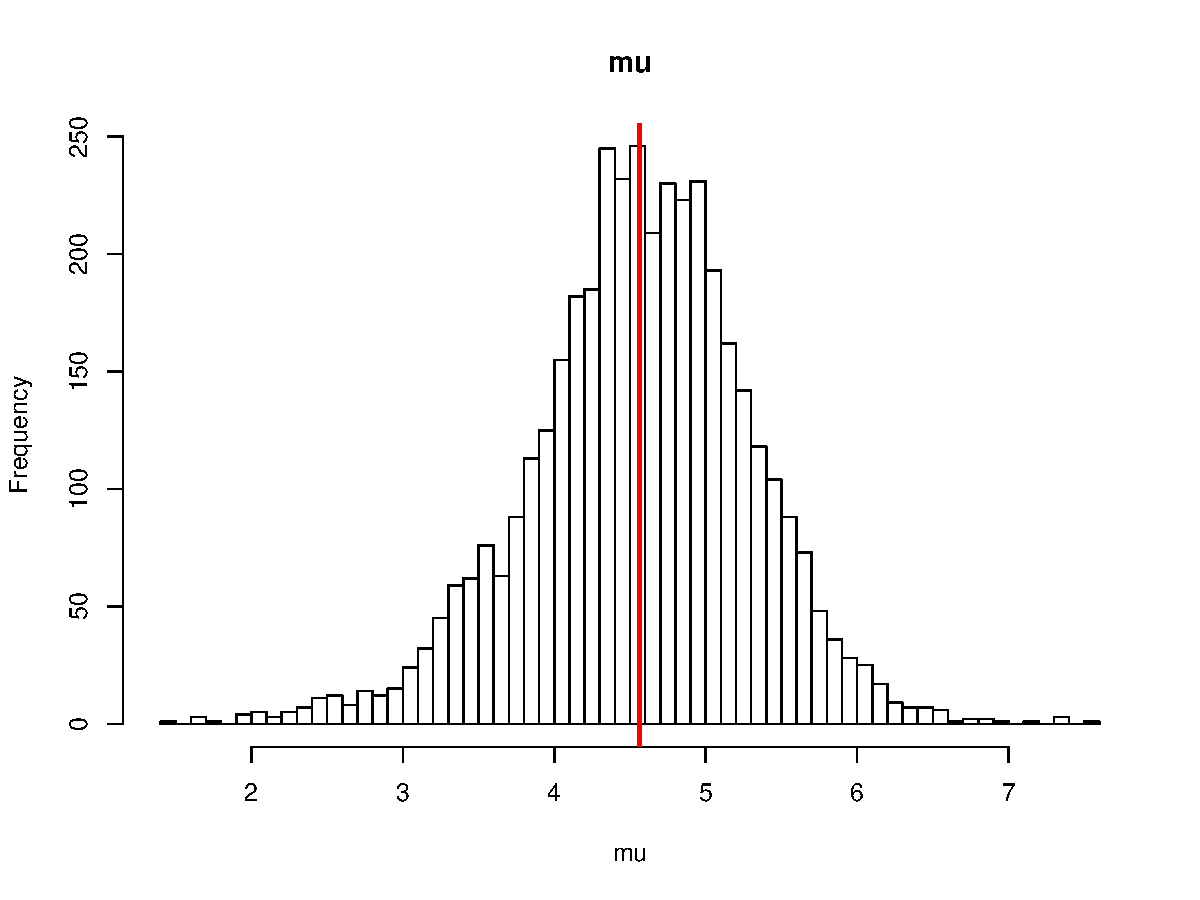
\includegraphics[trim={0cm 0cm 0cm 0cm}, clip, scale=0.4]{../figs/norm1_mu.pdf}
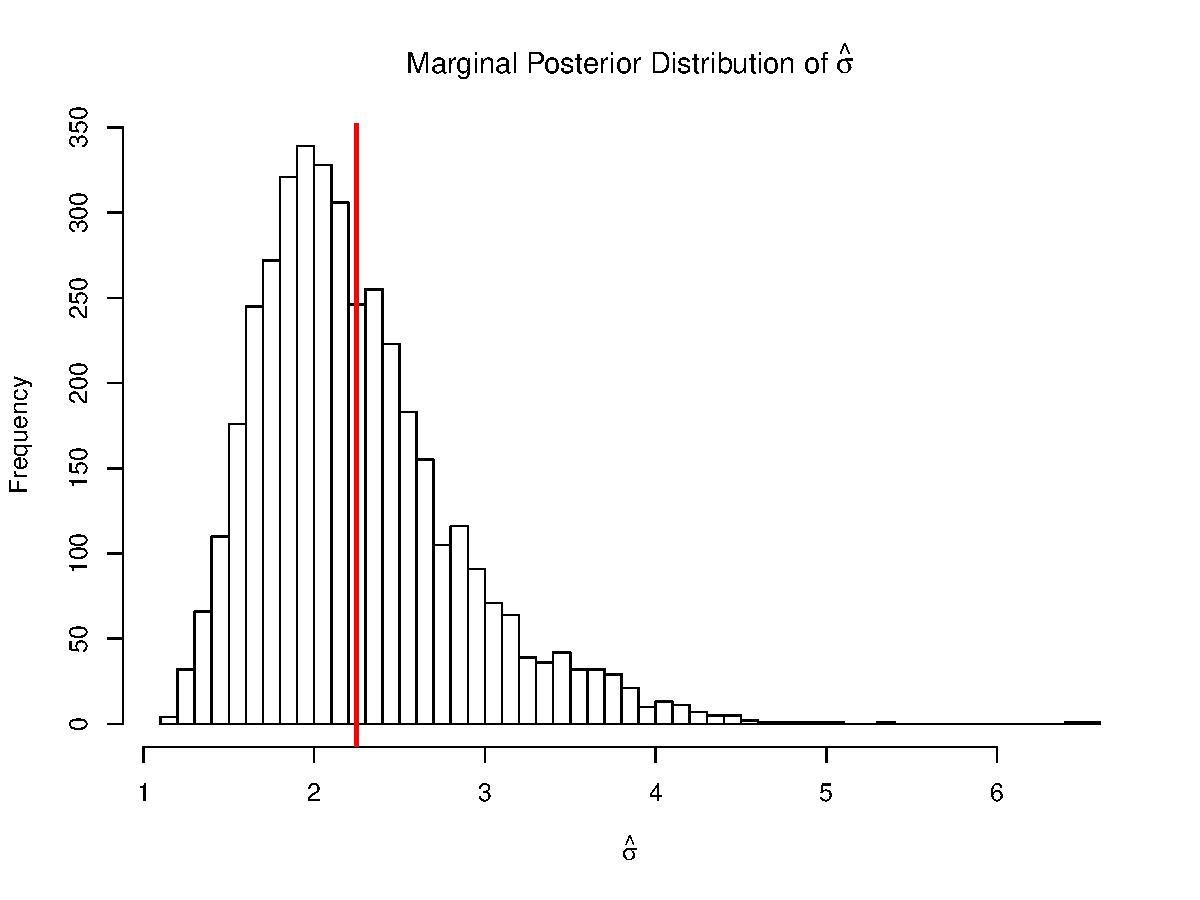
\includegraphics[trim={0cm 0cm 0cm 0cm}, clip, scale=0.4]{../figs/norm1_sigma.pdf}
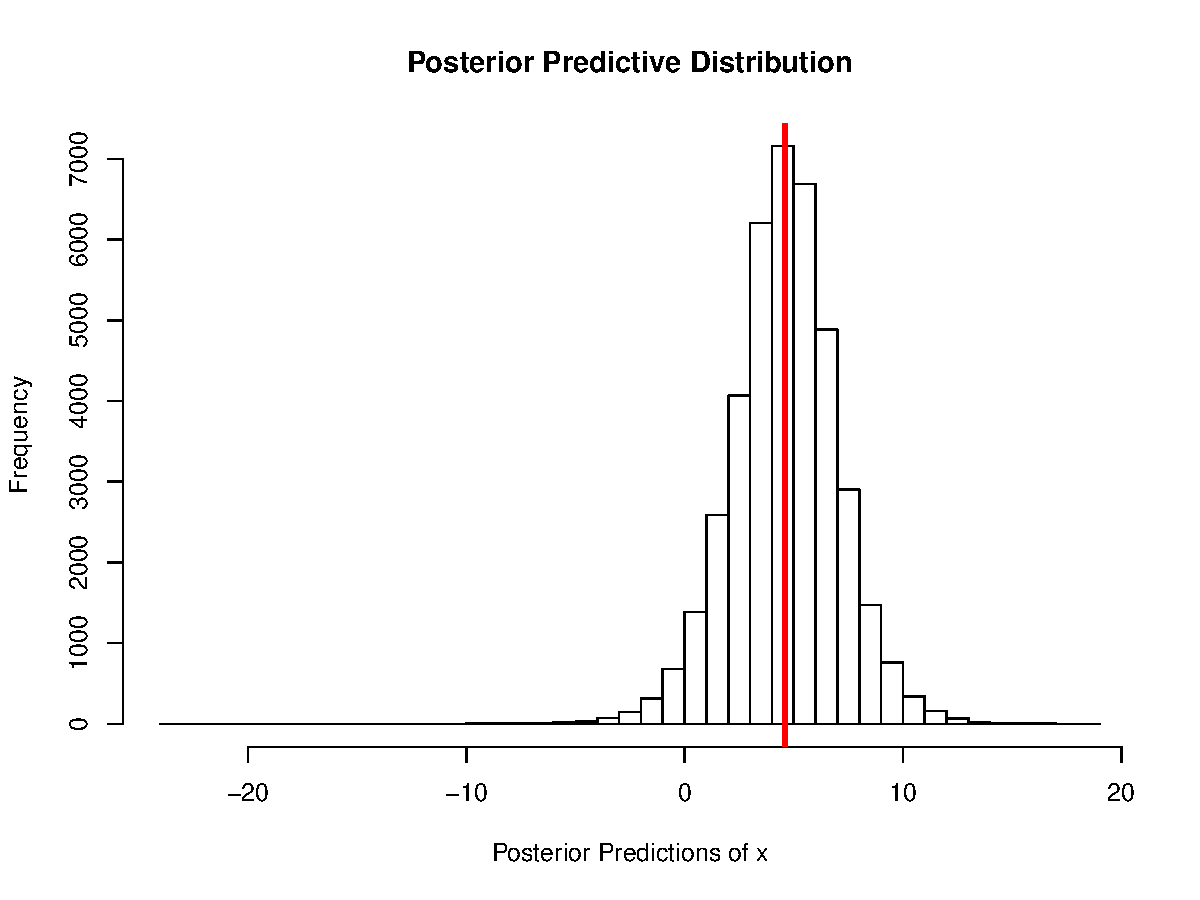
\includegraphics[trim={0cm 0cm 0cm 0cm}, clip, scale=0.4]{../figs/norm1_pp.pdf}
\footnotesize
\end{minipage}
\end{figure}

\noindent We are still interested in testing if the mean is different from the hypothesized value $\mu_0 = 4.5$. To do this we can compute quantiles with the posterior samples using probabilities defined by the researcher. These \emph{uncertainty intervals} enable us to communicate the probability that the estimated mean is between two values conditional on the data and prior information.\footnote{Uncertainty intervals are also known as credible intervals.}  The wider the interval, the more uncertainty we have about our estimate. The figure below illustrates the 50\% and 90\% uncertainty intervals for the location parameter. We identify that 90\% of the marginal posterior is between 3.3 and 5.7. It is at the discretion of the researcher to determine whether this interval is satisfactory to probabilistically conclude that the marginal posterior distribution of $\hat{\mu}$ is not different from 4.5. If the 90\% uncertainty interval excluded 4.5 then we could say that there is a 90\% chance that the mean estimated from the sample is different from 4.5. \\

\noindent An analogous approach to what we outlined above is to first take the difference between the samples $\hat{\mu}$ and the hypothesized value $\mu_0$. Then we can compute the quantiles in a similar fashion but would now be interested to know whether or not the 90\% interval contained zero (instead of the hypothesized value). If it does not then we can be 90\% sure that $\hat{\mu}$ is meaningfully different from $\mu_0$. If the interval does contain zero then the difference between $\mu_0$ and at least one of the samples was zero indicating that we cannot be 90\% sure that $\hat{\mu}$ is different from $\mu_0$. \\

\begin{figure}[H]\caption[]{Marginal posterior distribution of $\mu$}
\centering
\begin{minipage}{0.6\linewidth}
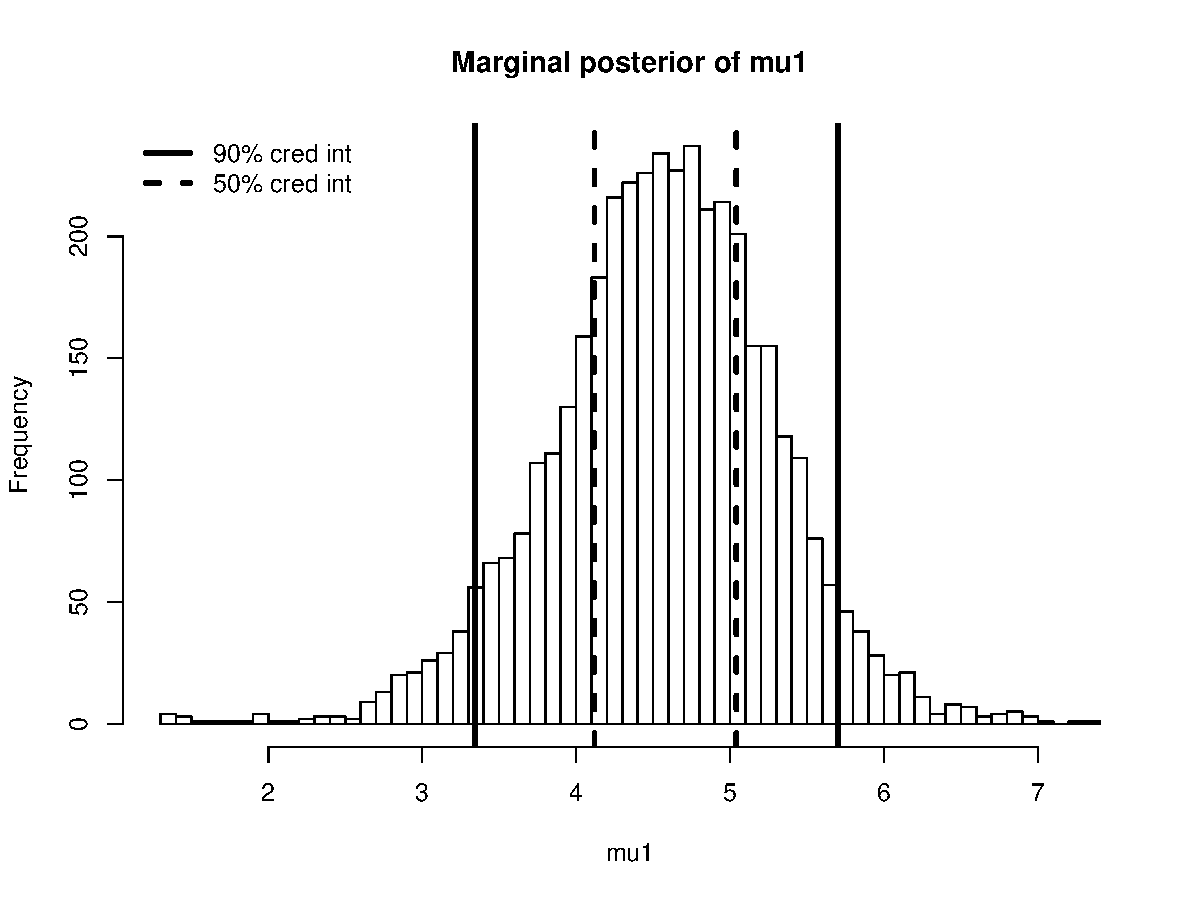
\includegraphics[trim={0cm 0cm 0cm 1.5cm}, clip, scale=0.6]{../figs/norm1.pdf}
\end{minipage}
\end{figure}

\section{Inference on (Posterior) Predictions}

\noindent Testing parameters does not tell us about the predictive capability of the model. It just allows us to make certain conclusions about the parameters in the model while assuming that the model itself is correct. In order to test whether the generative model is appropriate to model $x$ we need to perform inference on the posterior predictions.
One way to do this is to compute $\hat{x}-x$ along with the appropriate quantiles. In the figure below we plot the 90\% and 50\% uncertainty intervals for this difference. Notice that they contain zero (in fact the distribution is centered around zero). This indicates that most of the posterior predictions were close to the actual data. \\


\begin{figure}[H]\caption[]{Distribution of $\hat{x}-x$ (Good Generative Model)}
\centering
\begin{minipage}{0.6\linewidth}
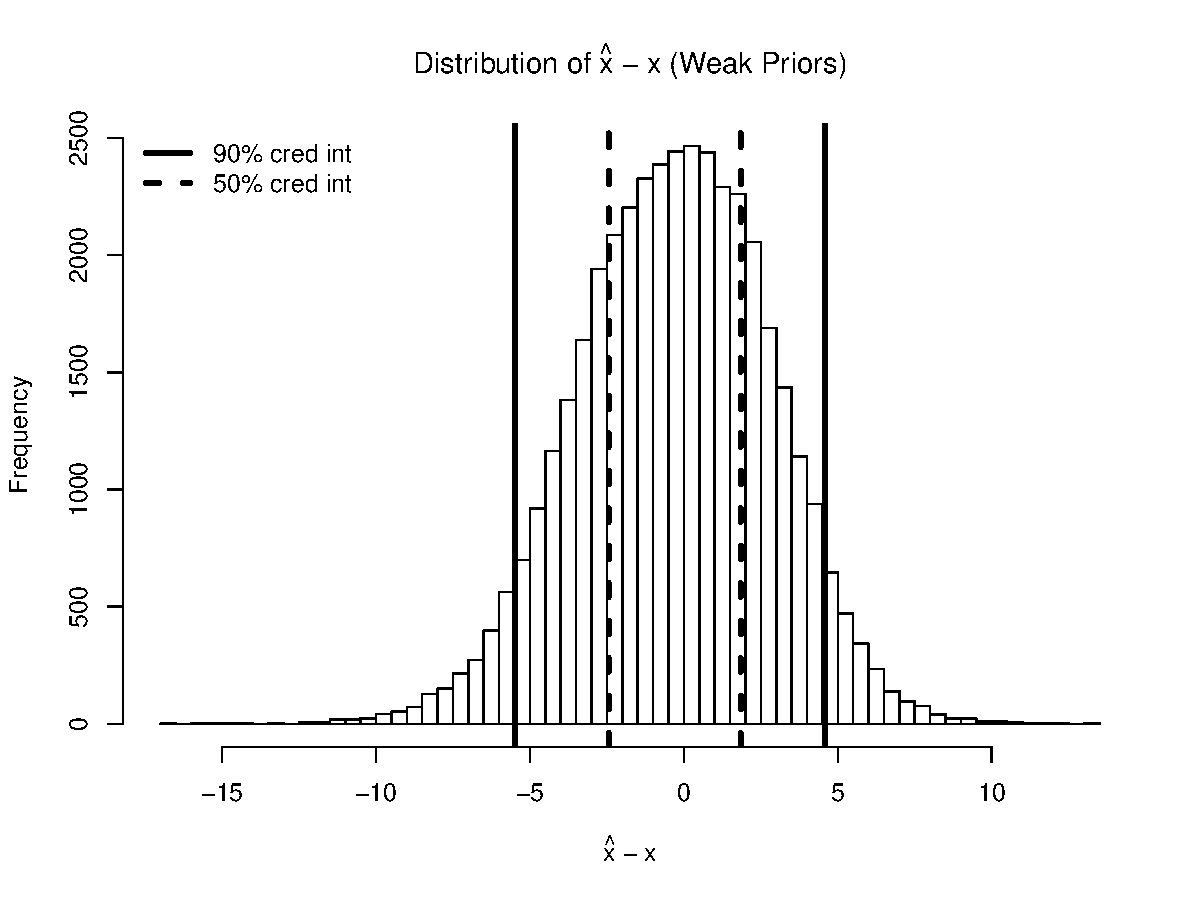
\includegraphics[trim={0cm 0cm 0cm 1.5cm}, clip, scale=0.5]{../figs/norm1_pp_diff.pdf}
\end{minipage}
\end{figure}

\noindent The figure below is an example of what the posterior predictive check would look like under an ill defined generative model. We use the same modeling structure as above but instead define informative priors on the parameters: $\hat{\mu} \sim \mathcal{N}(0,0.1)$ and $\hat{\sigma} \sim \mathcal{N}^{+}(0,0.1)$. Now the 90\% uncertainty interval no longer contains zero. This implies that we cannot be 90\% certain that the predictions match the data, so we cannot say that the model is a good representation of the data generation process. \\

\begin{figure}[H]\caption[]{Distribution of $\hat{x}-x$ (Bad Generative Model)}
\centering
\begin{minipage}{0.6\linewidth}
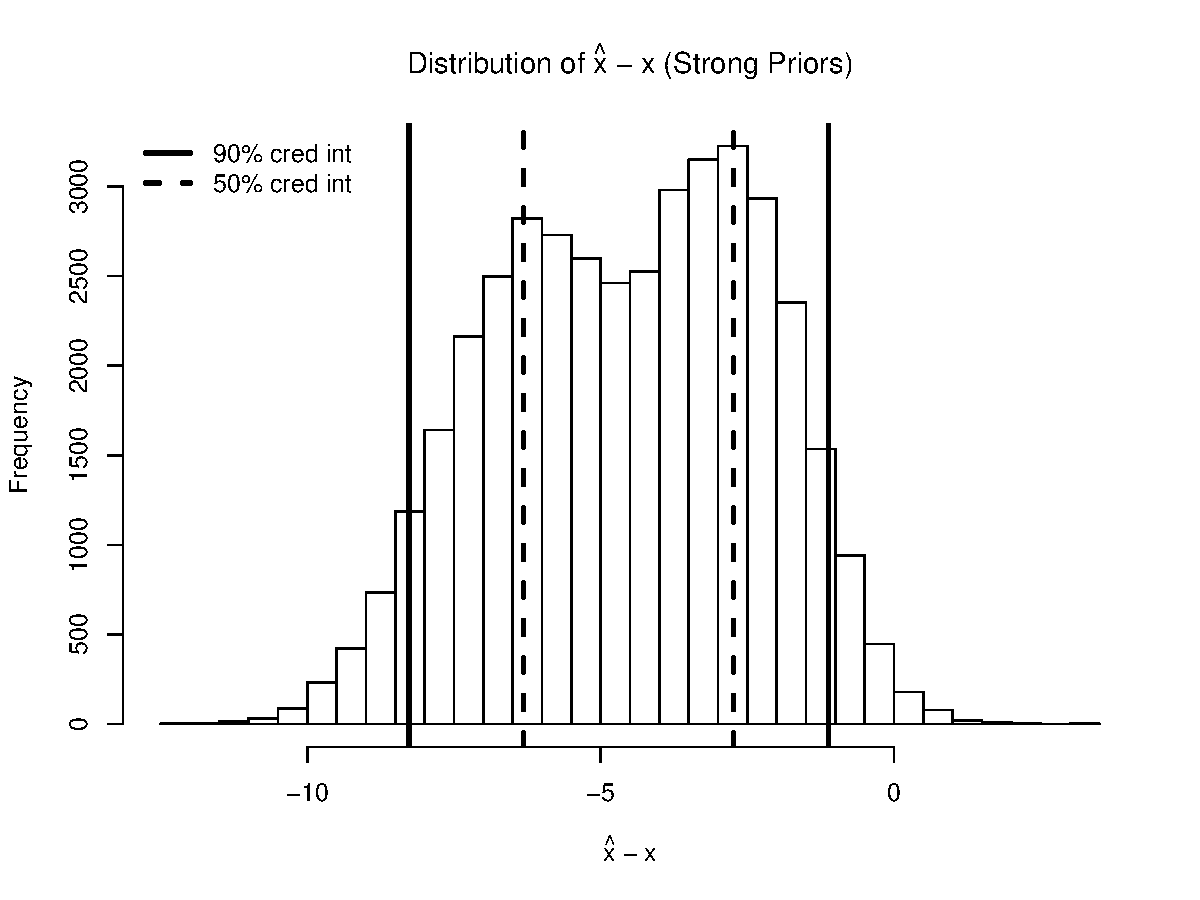
\includegraphics[trim={0cm 0cm 0cm 1.5cm}, clip, scale=0.5]{../figs/norm1_pp_diff_bad.pdf}
\end{minipage}
\end{figure}

\noindent In the ill defined model, if we focused only on inference on the parameter then we would have missed the fact that we specified a bad model given the data (in terms of predictive ability). This is crucial in the context of multivariate regression since the predictors and interactions may not be appropriate to model the outcome variable, and performing inference on regression parameters will overlook this. \\

\noindent It is important to note that a posterior predictive check helps determine whether the specified model is a good representation of the data generating process. In some cases the priors chosen might not lead to a posterior distribution that matches the actual data. In these situations it is up to the researcher to determine whether the prior beliefs should take precedence over having posterior predictions that match the data. \\

\section{Conclusion}

\noindent We have provided some clarity on what statistical significance means along with a feasible Bayesian alternative, as long as the researcher is willing to quantify and model prior beliefs. In addition to making inference easier for the researcher (since we directly deal with the parameter(s) of interest), the Bayesian approach should be make it easier to communicate the findings to non-statisticians since we are mostly dealing with probability instead of esoteric p-values or test statistics. \\

\noindent Aside from performing inference directly on parameters, an additional benefit with the Bayesian approach is that it enables researchers to quantify their prior information about the parameters in the model. This is particularly useful for small samples, where prior information has more influence than the likelihood of the data on the posterior distribution. With larger samples more informative priors need to be defined in order for them to have any substantial influence on the posterior distribution.

\pagebreak

\section{References}

\noindent Kozyrkov, Cassie. ``Statistician proves that statistics are boring.'' \emph{Medium}, 22 March 2019, \url{https://towardsdatascience.com/statistician-proves-that-statistics-are-boring-4fc22c95031b}. \\

\noindent Kruschke, John. ``Null Hypothesis Significance Testing.'' \emph{Doing Bayesian Data Analysis}, 2nd Edition, New York, Academic Press, 2015. \\

\noindent Stan Development Team. rstan: R interface to Stan. R package version 2.18.2, 2018. \\

\noindent Stan Development Team. RStanArm: Bayesian applied regression modeling via Stan. R package version 2.18.2, 2018. \\

\pagebreak

\section{Appendix A - Stan Code}

\noindent The one sample t-test model that was fit using rstanarm can also be fit in rstan by defining the following model in a Stan file:

\begin{verbatim}
               data {
                 int<lower=0> N;
                 vector[N] y;
                 real mu_loc;
                 real sigma_loc;
                 real<lower=0> mu_scale;
                 real<lower=0> sigma_scale;
               }
               parameters {
                 real mu;
                 real<lower=0> sigma;
               }
               model {
                 target+= normal_lpdf(y | mu, sigma);
                 target+= normal_lpdf(mu | mu_loc, mu_scale);
                 target+= normal_lpdf(sigma | sigma_loc, sigma_scale);
               }
               generated quantities {
                 real y_hat[N];
                 for (n in 1:N)
                   y_hat[n] = normal_rng(mu, sigma);
               }

\end{verbatim}

\pagebreak

\section{Appendix B - Bayesian Alternative to Two Sample t-Test}

The one-sample approach can be extended to two samples. Suppose we have three data sets ($x_1$, $x_2$, and $x_3$) generated from the normal distribution.

\begin{verbatim}
  x1 <- c(5.820883, 2.667825, 3.332511, 3.388233, 7.976444,
          5.925112, 6.465919, 7.064625, 3.012066, 2.771472)
  x2 <- c(6.329095, 4.575028, 1.346890, 6.440587, 7.479409,
          1.736296, 5.091112, 3.865324, 7.728403, 1.792258)
  x3 <- c(-2.541337, -2.778205, -1.363428, -4.821875, -2.526202,
          -3.587017, -1.073344, -2.400323,  3.287509,  3.278655)
\end{verbatim}

\noindent We want to determine whether the mean of $x_1$ is different from that of $x_2$ and $x_3$. Modeling each set of data according to the approach in the previous section gives the marginal posterior distributions for the location parameters ($\hat{\mu}_1$, $\hat{\mu}_2$, and $\hat{\mu}_3$). We can then compute the 50\% and 90\% quantiles for $\hat{\mu}_1 - \hat{\mu}_2$ and $\hat{\mu}_1 - \hat{\mu}_3$. For $\hat{\mu}_1 - \hat{\mu}_2$ we find that 90\% of the difference in location parameters is between -1.5 and 2.0. This interval contains zero, which means 90\% of the time we cannot confidently conclude that the means of the two samples, $x_1$ and $x_2$ are different. On the other hand the 90\% uncertainty interval for $\hat{\mu}_1 - \hat{\mu}_3$ is 4.0 and 7.8 so we can say that 90\% of the time there is a difference between the means of $x_1$ and $x_3$. The figure below illustrates the uncertainty interval for each of these cases.

\begin{figure}[H]\caption[]{Two-sample Inference on Location Parameters}
\begin{minipage}{1\linewidth}
  \centering
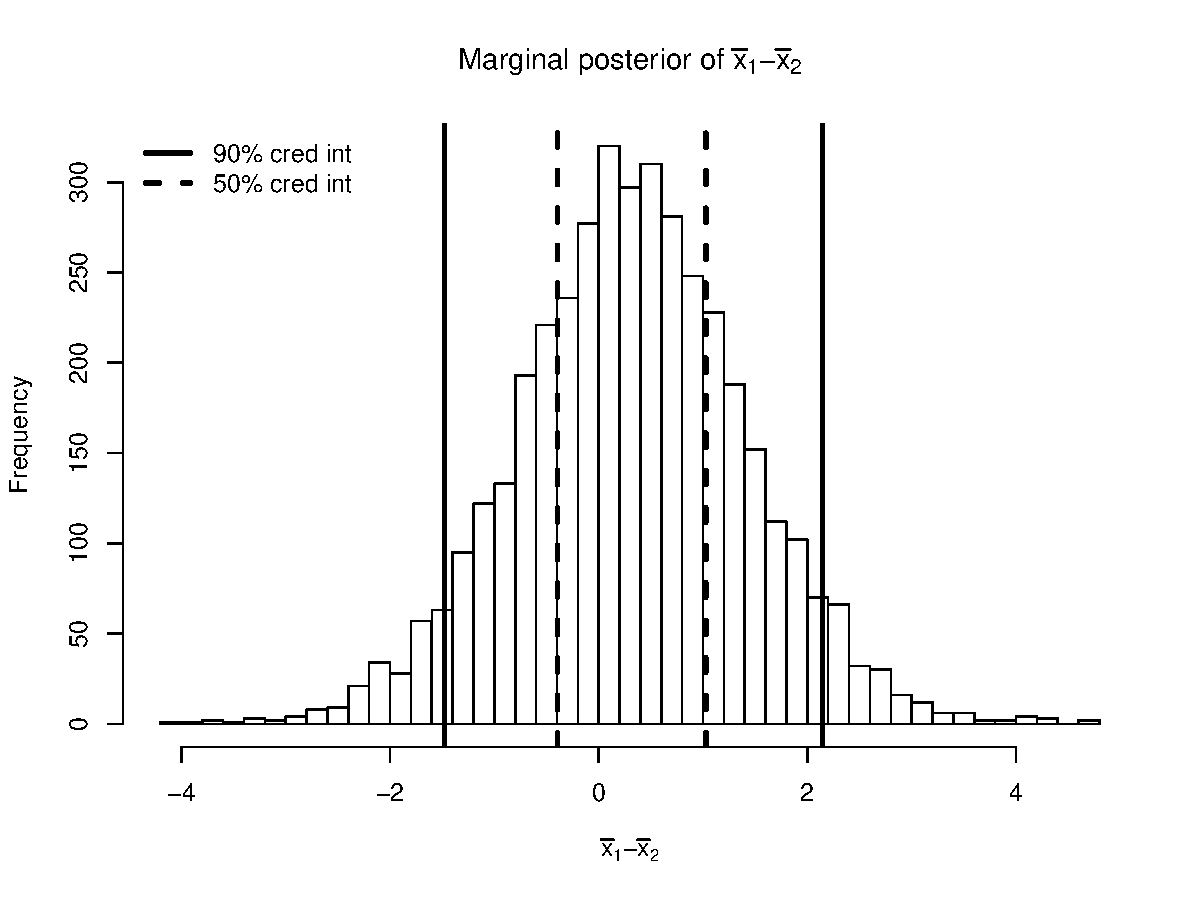
\includegraphics[trim={0cm 0cm 0cm 0cm}, clip, scale=0.4]{../figs/norm2.pdf}
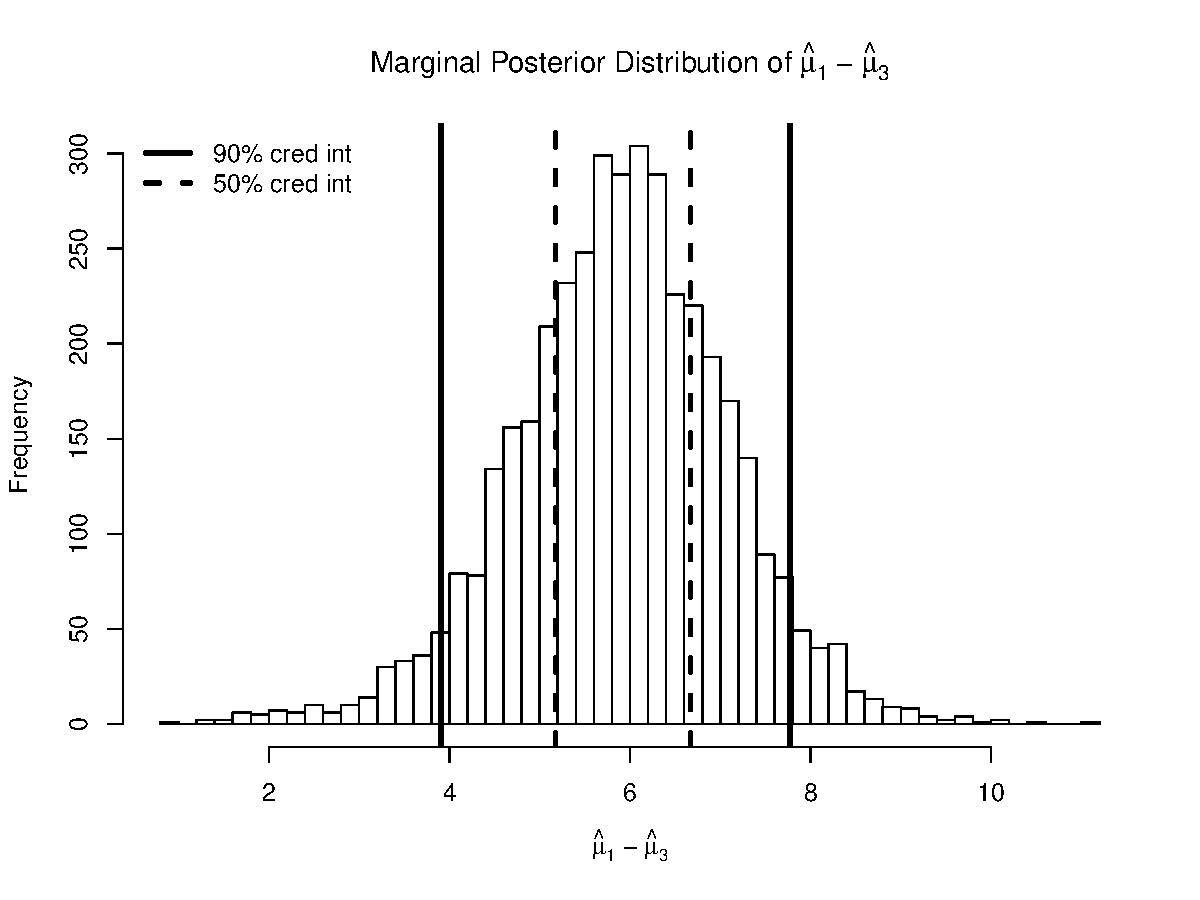
\includegraphics[trim={0cm 0cm 0cm 0cm}, clip, scale=0.4]{../figs/norm3.pdf}
\footnotesize
\end{minipage}
\end{figure}

\pagebreak

\section{Appendix C - Bayesian Alternative to Binomial test}

The example outlined above involves the t-test which requires the data to be noramally distributed. Here we look into inference on count data, specifically data generated from the binomial distribution. In Frequentist statistics the test used to compare the probability of success between some realized data sample and a hypothesized value is the \emph{binomial test}. This is commonly used in \textbf{A/B testing} where researchers are interested in the determining whether there is a substantial difference in the click through rate of an online advertising campaign. \\

\noindent In the context of the binomial test the p-value is calculated as,

\begin{align*}
d &= Bin(x, N, p_0) \\
\mbox{p-value} &= \sum_{k=0}^{N}Bin(k, N, p_0) \mbox{ s.t. } Bin(k, N, p_0) \leq d
\end{align*}

\noindent where $k$ is the number of successes, $x$ is the number of observed success (datum), $N$ is the number of trials, and $p_0$ is the hypothesized value for the probability of success. \\

\noindent As an example consider $x = 7$, $N = 10$, and $p_0 = 0.8$. Using the method described above we get a p-value of approximately 0.4296, preventing us from rejecting the null hypothesis that the probability of success is different from 0.8. This result is illustrated in the figure below which shows the density evaluated for each success under the hypothesized success rate. The densities that constitute the p-value are in red.

\begin{figure}[H]\caption[]{Empirical Distribution of t-Statistic}
\centering
\begin{minipage}{0.6\linewidth}
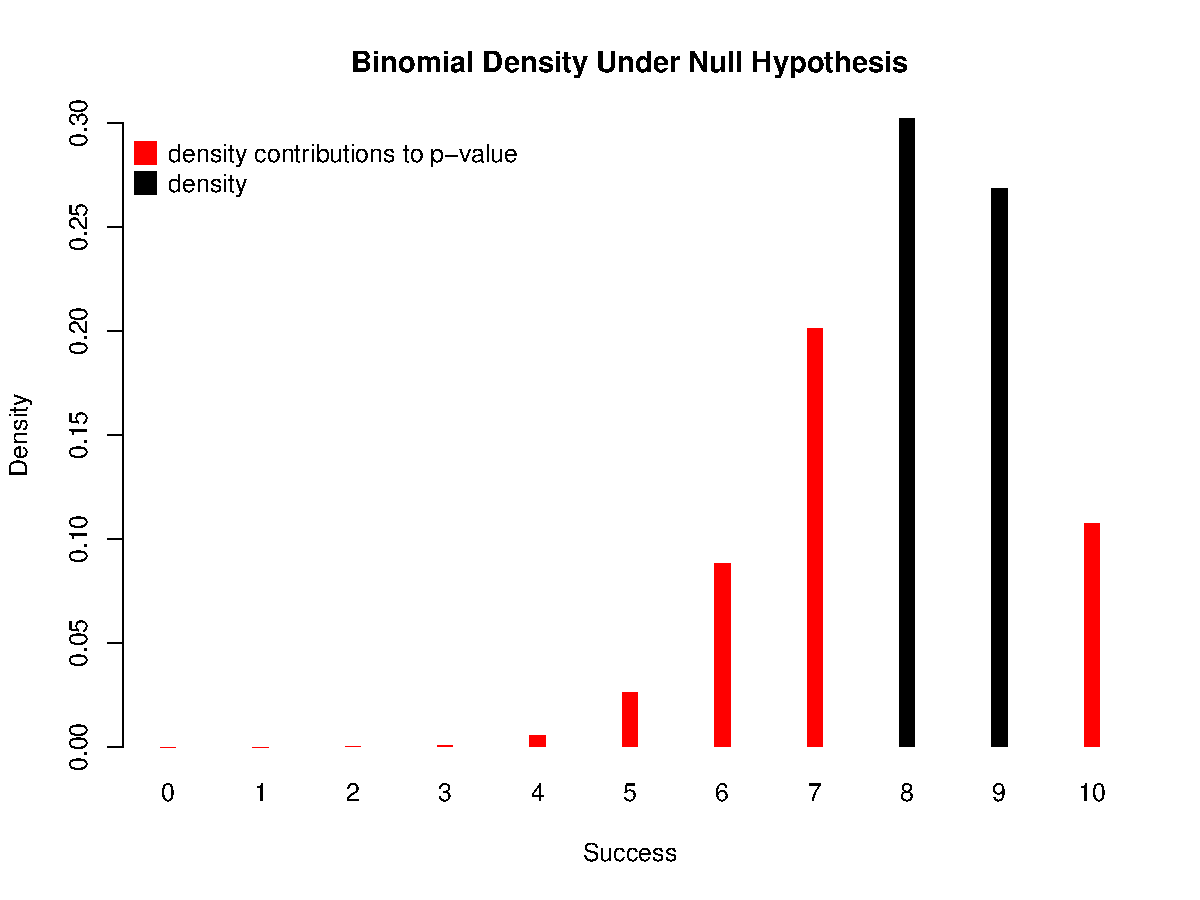
\includegraphics[trim={0cm 0cm 0cm 1.5cm}, clip, scale=0.6]{../figs/bintest_dist.pdf}
\end{minipage}
\end{figure}

\noindent As mentioned in this paper, the Bayesian approach involves modeling the data with prior information. In this case, the model is $7 \sim Bin(10, p)$ with a prior distribution defined on $p$ (the Beta distribution is typically used). We can then compute the quantiles and determine whether the estimated probability of success $p$ is different from the hypothesized value $p_0 = 0.8$. In this case we cannot conclude that the estimated probability of success is different from 0.8 since 90\% of the parameter samples are between 0.44 and 0.86, conditional on the data and prior information. This result is illustrated below. \\

\begin{figure}[H]\caption[]{Posterior Distribution of $p$}
\centering
\begin{minipage}{0.6\linewidth}
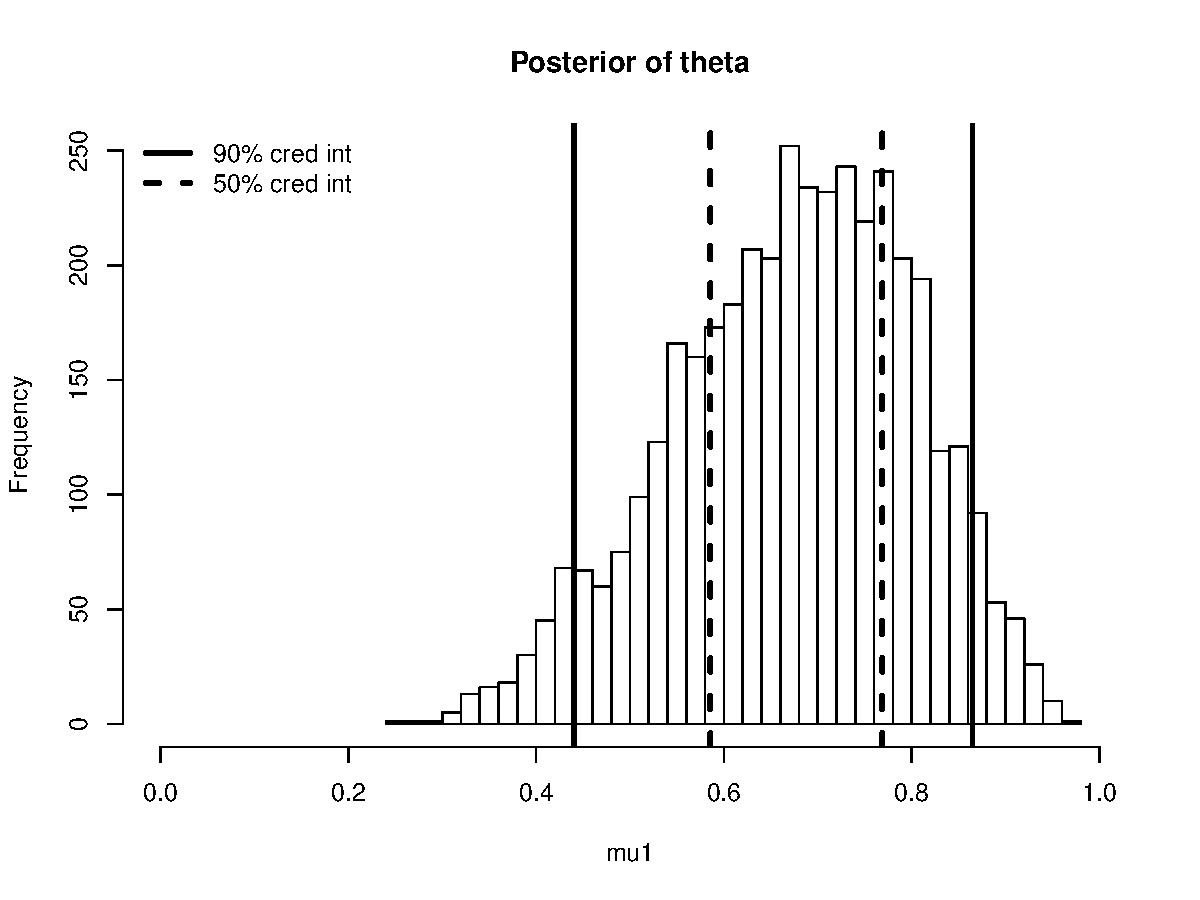
\includegraphics[trim={0cm 0cm 0cm 1.5cm}, clip, scale=0.6]{../figs/bin1.pdf}
\end{minipage}
\end{figure}

\noindent Note that the hypothesized value 0.8 is not in the 50\% credible interval (0.56, 0.78). This means that 50\% of the time the success rate parameter will be different from 0.8. It is up to the researcher to determine which interval is appropriate given the problem at hand. Under the context of the click through rate example, this would mean that there is a 50\% chance we will not observe a click through rate of 0.8.\\

\noindent This approach can easily be extended to multiple observations. The only difference would be to model the vector of successes (instead of a single observation) and a vector of associated trials. The inference on the probability of success parameter associated with these data would be the same. \\

\end{document}
